\documentclass[letterpaper]{article}

\usepackage{amsfonts}
\usepackage{amsmath}
\usepackage{graphicx}
\usepackage{hyperref}
\usepackage{tikz}

\begin{document}

\title{Approximately Euclidean Grids}
\author{Moshe Looks}

\maketitle

The distance $d_G(u, v)$ between vertices in an undirected graph $G = (V, E)$ is the number
of edges in a shortest path between $u$ and $v$. The distance $d_2(p, q)$ between points
Euclidean space is the $2$-norm of the line segment between $u$ and $v$. In two or more
dimensions, no injective mapping $f : V \to \mathbb{N}^2$ can satisfy $d_G(u, v) = d_2(f(u),
f(v))$ because of the incommensurability of the side and diagonal of the square. Nonetheless,
$d_G(u, v)$ can be used to approximate $d_2(f(u), f(v))$; the approximation will be better or
worse depending on our choices of $G$ and $f$. How well can $d_G$ approximate $d_2$, assuming
$|V| = N$?

This is an interesting question, but difficult to answer in full generality. Let's consider
the special case of a graph with $N = n^2$ vertices, arranged in a square grid to correspond
to the points $\{1, \ldots, n\} \times \{1, \ldots, n\}$. If we add edges between horizontal
and vertical neighbors, we get Manhattan distances ($d_1$, based on the $1$-norm). If we
additionally add edges between diagonal neighbors,\footnote{Without loss of generality, we
only consider diagonals corresponding to line segments of the form $\{p + (\Delta, \Delta) \,
| \, 0 \leq \Delta \leq 1\}$, and distances between vertices placed at pairs of points of the
form $(p, p + \Delta) \, | \, p, \Delta _\in \mathbb{N}^2$.} then we get chessboard distances
($d_\infty$, based on the $\infty$-norm).

\setlength{\tabcolsep}{15pt}
\begin{tabular}{ l r}
  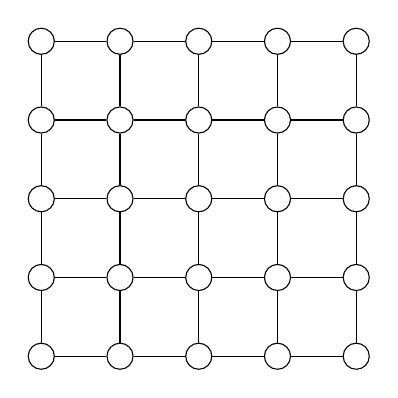
\begin{tikzpicture}
  \node (1x1) at (0, 0) [shape=circle, draw] {};
  \node (2x1) at (0, 1) [shape=circle, draw] {};
  \node (3x1) at (0, 2) [shape=circle, draw] {};
  \node (4x1) at (0, 3) [shape=circle, draw] {};
  \node (5x1) at (0, 4) [shape=circle, draw] {};
  \node (1x2) at (1, 0) [shape=circle, draw] {};
  \node (2x2) at (1, 1) [shape=circle, draw] {};
  \node (3x2) at (1, 2) [shape=circle, draw] {};
  \node (4x2) at (1, 3) [shape=circle, draw] {};
  \node (5x2) at (1, 4) [shape=circle, draw] {};
  \node (1x3) at (2, 0) [shape=circle, draw] {};
  \node (2x3) at (2, 1) [shape=circle, draw] {};
  \node (3x3) at (2, 2) [shape=circle, draw] {};
  \node (4x3) at (2, 3) [shape=circle, draw] {};
  \node (5x3) at (2, 4) [shape=circle, draw] {};
  \node (1x4) at (3, 0) [shape=circle, draw] {};
  \node (2x4) at (3, 1) [shape=circle, draw] {};
  \node (3x4) at (3, 2) [shape=circle, draw] {};
  \node (4x4) at (3, 3) [shape=circle, draw] {};
  \node (5x4) at (3, 4) [shape=circle, draw] {};
  \node (1x5) at (4, 0) [shape=circle, draw] {};
  \node (2x5) at (4, 1) [shape=circle, draw] {};
  \node (3x5) at (4, 2) [shape=circle, draw] {};
  \node (4x5) at (4, 3) [shape=circle, draw] {};
  \node (5x5) at (4, 4) [shape=circle, draw] {};
  \draw (1x1) -- (1x2);
  \draw (2x1) -- (2x2);
  \draw (3x1) -- (3x2);
  \draw (4x1) -- (4x2);
  \draw (5x1) -- (5x2);
  \draw (1x2) -- (1x3);
  \draw (2x2) -- (2x3);
  \draw (3x2) -- (3x3);
  \draw (4x2) -- (4x3);
  \draw (5x2) -- (5x3);
  \draw (1x3) -- (1x4);
  \draw (2x3) -- (2x4);
  \draw (3x3) -- (3x4);
  \draw (4x3) -- (4x4);
  \draw (5x3) -- (5x4);
  \draw (1x4) -- (1x5);
  \draw (2x4) -- (2x5);
  \draw (3x4) -- (3x5);
  \draw (4x4) -- (4x5);
  \draw (5x4) -- (5x5);
  \draw (1x1) -- (2x1);
  \draw (2x1) -- (3x1);
  \draw (3x1) -- (4x1);
  \draw (4x1) -- (5x1);
  \draw (1x2) -- (2x2);
  \draw (2x2) -- (3x2);
  \draw (3x2) -- (4x2);
  \draw (4x2) -- (5x2);
  \draw (1x3) -- (2x3);
  \draw (2x3) -- (3x3);
  \draw (3x3) -- (4x3);
  \draw (4x3) -- (5x3);
  \draw (1x4) -- (2x4);
  \draw (2x4) -- (3x4);
  \draw (3x4) -- (4x4);
  \draw (4x4) -- (5x4);
  \draw (1x5) -- (2x5);
  \draw (2x5) -- (3x5);
  \draw (3x5) -- (4x5);
  \draw (4x5) -- (5x5);
\end{tikzpicture}
 & 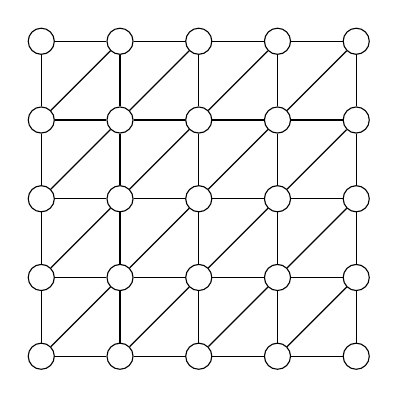
\begin{tikzpicture}
  \node (1x1) at (0, 0) [shape=circle, draw] {};
  \node (2x1) at (0, 1) [shape=circle, draw] {};
  \node (3x1) at (0, 2) [shape=circle, draw] {};
  \node (4x1) at (0, 3) [shape=circle, draw] {};
  \node (5x1) at (0, 4) [shape=circle, draw] {};
  \node (1x2) at (1, 0) [shape=circle, draw] {};
  \node (2x2) at (1, 1) [shape=circle, draw] {};
  \node (3x2) at (1, 2) [shape=circle, draw] {};
  \node (4x2) at (1, 3) [shape=circle, draw] {};
  \node (5x2) at (1, 4) [shape=circle, draw] {};
  \node (1x3) at (2, 0) [shape=circle, draw] {};
  \node (2x3) at (2, 1) [shape=circle, draw] {};
  \node (3x3) at (2, 2) [shape=circle, draw] {};
  \node (4x3) at (2, 3) [shape=circle, draw] {};
  \node (5x3) at (2, 4) [shape=circle, draw] {};
  \node (1x4) at (3, 0) [shape=circle, draw] {};
  \node (2x4) at (3, 1) [shape=circle, draw] {};
  \node (3x4) at (3, 2) [shape=circle, draw] {};
  \node (4x4) at (3, 3) [shape=circle, draw] {};
  \node (5x4) at (3, 4) [shape=circle, draw] {};
  \node (1x5) at (4, 0) [shape=circle, draw] {};
  \node (2x5) at (4, 1) [shape=circle, draw] {};
  \node (3x5) at (4, 2) [shape=circle, draw] {};
  \node (4x5) at (4, 3) [shape=circle, draw] {};
  \node (5x5) at (4, 4) [shape=circle, draw] {};
  \draw (1x1) -- (1x2);
  \draw (2x1) -- (2x2);
  \draw (3x1) -- (3x2);
  \draw (4x1) -- (4x2);
  \draw (5x1) -- (5x2);
  \draw (1x2) -- (1x3);
  \draw (2x2) -- (2x3);
  \draw (3x2) -- (3x3);
  \draw (4x2) -- (4x3);
  \draw (5x2) -- (5x3);
  \draw (1x3) -- (1x4);
  \draw (2x3) -- (2x4);
  \draw (3x3) -- (3x4);
  \draw (4x3) -- (4x4);
  \draw (5x3) -- (5x4);
  \draw (1x4) -- (1x5);
  \draw (2x4) -- (2x5);
  \draw (3x4) -- (3x5);
  \draw (4x4) -- (4x5);
  \draw (5x4) -- (5x5);
  \draw (1x1) -- (2x1);
  \draw (2x1) -- (3x1);
  \draw (3x1) -- (4x1);
  \draw (4x1) -- (5x1);
  \draw (1x2) -- (2x2);
  \draw (2x2) -- (3x2);
  \draw (3x2) -- (4x2);
  \draw (4x2) -- (5x2);
  \draw (1x3) -- (2x3);
  \draw (2x3) -- (3x3);
  \draw (3x3) -- (4x3);
  \draw (4x3) -- (5x3);
  \draw (1x4) -- (2x4);
  \draw (2x4) -- (3x4);
  \draw (3x4) -- (4x4);
  \draw (4x4) -- (5x4);
  \draw (1x5) -- (2x5);
  \draw (2x5) -- (3x5);
  \draw (3x5) -- (4x5);
  \draw (4x5) -- (5x5);
  \draw (1x1) -- (2x2);
  \draw (2x1) -- (3x2);
  \draw (3x1) -- (4x2);
  \draw (4x1) -- (5x2);
  \draw (1x2) -- (2x3);
  \draw (2x2) -- (3x3);
  \draw (3x2) -- (4x3);
  \draw (4x2) -- (5x3);
  \draw (1x3) -- (2x4);
  \draw (2x3) -- (3x4);
  \draw (3x3) -- (4x4);
  \draw (4x3) -- (5x4);
  \draw (1x4) -- (2x5);
  \draw (2x4) -- (3x5);
  \draw (3x4) -- (4x5);
  \draw (4x4) -- (5x5);
\end{tikzpicture}

\end{tabular}

We have the nice property that $d_1(p, q) \leq d_2(p, q) \leq d_\infty(p, q)$, but
nonetheless, neither one of these constructs gives us a very good approximation of
$d_2$. Indeed, it is easy to see that the divergences from $d_2$ grow unboundedly with $n$.
In fact, Tobias Fritz has \href{https://arxiv.org/abs/1109.1963}{proven} that this divergence
happens for \emph{every} distance function based on periodic graph. But nothing prevents us
from considering aperiodic graphs. What happens if we start with a graph corresponding to
$d_1$ and we add edges between only \emph{some} diagonal neighbors?

\section{An overly simplistic approach}

In the spirit of trying simple things first, lets see what happens if we take a greedy
approach and only consider distance to $\mathbf{1} = (1, 1)$. It can be easily seen that
if there is an edge between the vertices corresponding to points $(i, j)$ and $(i + 1, j+1)$
then
\begin{equation}
  d_G(\mathbf{1}, (i+1, j+1)) = 1 + d_G(\mathbf{1}, (i, j))
\end{equation}
and that otherwise
\begin{equation}
  d_G(\mathbf{1}, (i+1, j+1)) = 1 + \min(d_G(\mathbf{1}, (i + 1, j)),
                                         d_G(\mathbf{1}, (i, j + 1)))
\end{equation}

This suggests simply


This approach gives us very nice circular arcs around $\mathbf{1}$

\includegraphics[scale=0.2]{cs.png}

But very ugly circular arcs around other vertices.

\includegraphics[scale=0.2]{cs2.png}

We can generalize this approach and consider distances to all $\mathbf{1}$ but also

for example:

\begin{center}
  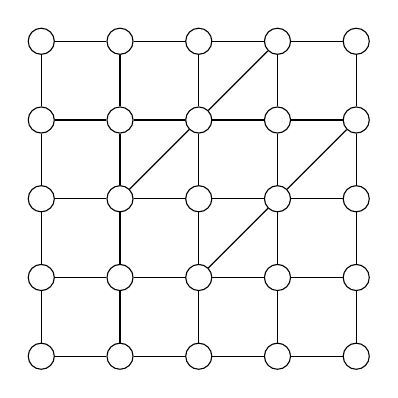
\begin{tikzpicture}
  \node (1x1) at (0, 0) [shape=circle, draw] {};
  \node (2x1) at (0, 1) [shape=circle, draw] {};
  \node (3x1) at (0, 2) [shape=circle, draw] {};
  \node (4x1) at (0, 3) [shape=circle, draw] {};
  \node (5x1) at (0, 4) [shape=circle, draw] {};
  \node (1x2) at (1, 0) [shape=circle, draw] {};
  \node (2x2) at (1, 1) [shape=circle, draw] {};
  \node (3x2) at (1, 2) [shape=circle, draw] {};
  \node (4x2) at (1, 3) [shape=circle, draw] {};
  \node (5x2) at (1, 4) [shape=circle, draw] {};
  \node (1x3) at (2, 0) [shape=circle, draw] {};
  \node (2x3) at (2, 1) [shape=circle, draw] {};
  \node (3x3) at (2, 2) [shape=circle, draw] {};
  \node (4x3) at (2, 3) [shape=circle, draw] {};
  \node (5x3) at (2, 4) [shape=circle, draw] {};
  \node (1x4) at (3, 0) [shape=circle, draw] {};
  \node (2x4) at (3, 1) [shape=circle, draw] {};
  \node (3x4) at (3, 2) [shape=circle, draw] {};
  \node (4x4) at (3, 3) [shape=circle, draw] {};
  \node (5x4) at (3, 4) [shape=circle, draw] {};
  \node (1x5) at (4, 0) [shape=circle, draw] {};
  \node (2x5) at (4, 1) [shape=circle, draw] {};
  \node (3x5) at (4, 2) [shape=circle, draw] {};
  \node (4x5) at (4, 3) [shape=circle, draw] {};
  \node (5x5) at (4, 4) [shape=circle, draw] {};
  \draw (1x1) -- (1x2);
  \draw (2x1) -- (2x2);
  \draw (3x1) -- (3x2);
  \draw (4x1) -- (4x2);
  \draw (5x1) -- (5x2);
  \draw (1x2) -- (1x3);
  \draw (2x2) -- (2x3);
  \draw (3x2) -- (3x3);
  \draw (4x2) -- (4x3);
  \draw (5x2) -- (5x3);
  \draw (1x3) -- (1x4);
  \draw (2x3) -- (2x4);
  \draw (3x3) -- (3x4);
  \draw (4x3) -- (4x4);
  \draw (5x3) -- (5x4);
  \draw (1x4) -- (1x5);
  \draw (2x4) -- (2x5);
  \draw (3x4) -- (3x5);
  \draw (4x4) -- (4x5);
  \draw (5x4) -- (5x5);
  \draw (1x1) -- (2x1);
  \draw (2x1) -- (3x1);
  \draw (3x1) -- (4x1);
  \draw (4x1) -- (5x1);
  \draw (1x2) -- (2x2);
  \draw (2x2) -- (3x2);
  \draw (3x2) -- (4x2);
  \draw (4x2) -- (5x2);
  \draw (1x3) -- (2x3);
  \draw (2x3) -- (3x3);
  \draw (3x3) -- (4x3);
  \draw (4x3) -- (5x3);
  \draw (1x4) -- (2x4);
  \draw (2x4) -- (3x4);
  \draw (3x4) -- (4x4);
  \draw (4x4) -- (5x4);
  \draw (1x5) -- (2x5);
  \draw (2x5) -- (3x5);
  \draw (3x5) -- (4x5);
  \draw (4x5) -- (5x5);
  \draw (3x2) -- (4x3);
  \draw (2x3) -- (3x4);
  \draw (4x3) -- (5x4);
  \draw (3x4) -- (4x5);
\end{tikzpicture}

\end{center}

This graph has an interesting property; for every Pythagorean triple\footnote{Triples of
natural numbers $(a, b, c)$ s.t. $a^2 + b^2 = c^2$; eg. $(3, 4, 5)$, $(12, 5, 13)$, \&c.}
$(a, b, c)$ and every pair of vertices $(p, q)$ corresponding respectively to $(x, y)$ and
$(x + a, y + b)$, $d(p, q) = c$. Let's call an undirected graph with $|V| = n^2$ that has
this property an order-$n$ Eugrid (Euclidean grid).

Pythagorean triples are dense in the rational numbers. Consequently, a Eugrid of sufficiently
high order would, in a certain sense, perfectly reflect the structure of Euclidean space, insofar as
it is \emph{can} be reflected by a finite square grid. But do high-order Eugrids
exist?\footnote{Spoiler: they do not.}

\section{Answering the Question}

We can construct a state space to search for order-$n$ Eugrids by putting undirected graphs
in correspondence with $(n - 1) \times (n - 1)$ bit matrices where $1$s correspond to the
presence of edges between diagonal neighbors.\footnote{Eugrids include all edges between
horizontal and vertical neighbors, by definition.} For example, the order-$5$ Eugrid
exhibited above corresponds to a $4 x 4$ Eugridean matrix:

\begin{equation*}
\begin{matrix}
  0 & 0 & 0 & 0 \\
  0 & 0 & 1 & 0 \\
  0 & 1 & 0 & 1 \\
  0 & 0 & 1 & 0
\end{matrix}
\end{equation*}

The state space for order $n$ has $2^{(n-1)^2}$ elements. For $n=5$ this is only 65,536 and
we can brute-force it to see that there are 10,948 order-$5$ Eugrids; they are rather thick
on the ground. What to do about higher orders where exponential growth makes things
unpleasant? We can make some headway by noticing that higher-order Eugrids must be composed
of lower-order ones. In particular, if matrix $\mathbf{A}$ corresponds to an order-$n$
Eugrid, then all submatrices $\mathbf{A}_{1:m,1:m}$ correspond to order-$m$ Eugrids.

This naturally suggests a partition of the full $(n-1)^2$-dimensional state space into
$(n-1)$ disjoint ``layers'', like so:

\begin{center}
  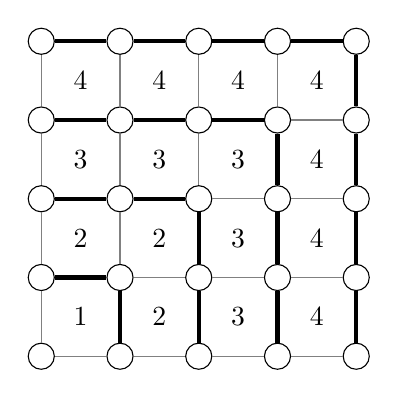
\begin{tikzpicture}
  \node (1x1) at (0, 0) [shape=circle, draw] {};
  \node (2x1) at (0, 1) [shape=circle, draw] {};
  \node (3x1) at (0, 2) [shape=circle, draw] {};
  \node (4x1) at (0, 3) [shape=circle, draw] {};
  \node (5x1) at (0, 4) [shape=circle, draw] {};
  \node (1x2) at (1, 0) [shape=circle, draw] {};
  \node (2x2) at (1, 1) [shape=circle, draw] {};
  \node (3x2) at (1, 2) [shape=circle, draw] {};
  \node (4x2) at (1, 3) [shape=circle, draw] {};
  \node (5x2) at (1, 4) [shape=circle, draw] {};
  \node (1x3) at (2, 0) [shape=circle, draw] {};
  \node (2x3) at (2, 1) [shape=circle, draw] {};
  \node (3x3) at (2, 2) [shape=circle, draw] {};
  \node (4x3) at (2, 3) [shape=circle, draw] {};
  \node (5x3) at (2, 4) [shape=circle, draw] {};
  \node (1x4) at (3, 0) [shape=circle, draw] {};
  \node (2x4) at (3, 1) [shape=circle, draw] {};
  \node (3x4) at (3, 2) [shape=circle, draw] {};
  \node (4x4) at (3, 3) [shape=circle, draw] {};
  \node (5x4) at (3, 4) [shape=circle, draw] {};
  \node (1x5) at (4, 0) [shape=circle, draw] {};
  \node (2x5) at (4, 1) [shape=circle, draw] {};
  \node (3x5) at (4, 2) [shape=circle, draw] {};
  \node (4x5) at (4, 3) [shape=circle, draw] {};
  \node (5x5) at (4, 4) [shape=circle, draw] {};
  \draw[thin, gray] (1x1) -- (1x2);
  \draw[ultra thick] (2x1) -- (2x2);
  \draw[ultra thick] (3x1) -- (3x2);
  \draw[ultra thick] (4x1) -- (4x2);
  \draw[ultra thick] (5x1) -- (5x2);
  \draw[thin, gray] (1x2) -- (1x3);
  \draw[thin, gray] (2x2) -- (2x3);
  \draw[ultra thick] (3x2) -- (3x3);
  \draw[ultra thick] (4x2) -- (4x3);
  \draw[ultra thick] (5x2) -- (5x3);
  \draw[thin, gray] (1x3) -- (1x4);
  \draw[thin, gray] (2x3) -- (2x4);
  \draw[thin, gray] (3x3) -- (3x4);
  \draw[ultra thick] (4x3) -- (4x4);
  \draw[ultra thick] (5x3) -- (5x4);
  \draw[thin, gray] (1x4) -- (1x5);
  \draw[thin, gray] (2x4) -- (2x5);
  \draw[thin, gray] (3x4) -- (3x5);
  \draw[thin, gray] (4x4) -- (4x5);
  \draw[ultra thick] (5x4) -- (5x5);
  \draw[thin, gray] (1x1) -- (2x1);
  \draw[thin, gray] (2x1) -- (3x1);
  \draw[thin, gray] (3x1) -- (4x1);
  \draw[thin, gray] (4x1) -- (5x1);
  \draw[ultra thick] (1x2) -- (2x2);
  \draw[thin, gray] (2x2) -- (3x2);
  \draw[thin, gray] (3x2) -- (4x2);
  \draw[thin, gray] (4x2) -- (5x2);
  \draw[ultra thick] (1x3) -- (2x3);
  \draw[ultra thick] (2x3) -- (3x3);
  \draw[thin, gray] (3x3) -- (4x3);
  \draw[thin, gray] (4x3) -- (5x3);
  \draw[ultra thick] (1x4) -- (2x4);
  \draw[ultra thick] (2x4) -- (3x4);
  \draw[ultra thick] (3x4) -- (4x4);
  \draw[thin, gray] (4x4) -- (5x4);
  \draw[ultra thick] (1x5) -- (2x5);
  \draw[ultra thick] (2x5) -- (3x5);
  \draw[ultra thick] (3x5) -- (4x5);
  \draw[ultra thick] (4x5) -- (5x5);
\node at (0.5, 0.5) {1};
\node at (0.5, 1.5) {2};
\node at (1.5, 0.5) {2};
\node at (1.5, 1.5) {2};
\node at (0.5, 2.5) {3};
\node at (1.5, 2.5) {3};
\node at (2.5, 0.5) {3};
\node at (2.5, 1.5) {3};
\node at (2.5, 2.5) {3};
\node at (0.5, 3.5) {4};
\node at (1.5, 3.5) {4};
\node at (2.5, 3.5) {4};
\node at (3.5, 0.5) {4};
\node at (3.5, 1.5) {4};
\node at (3.5, 2.5) {4};
\node at (3.5, 3.5) {4};
\end{tikzpicture}

\end{center}

Possible diagonals for the $m$th layer correspond to squares numbered $m$. So rather than
constructing an entire state in one go, we only ever construct substates corresponding to
individual layers. When constructing a substate corresponding to layer $m+1$, we can assume
that all substates corresponding to layers $1 \ldots m$ are valid (i.e. correspond to
lower-order Eugrids). We may have to backtrack of course; some lower-order Eugrids are dead
ends.

This is a good start towards tractability but is insufficient; the state subspace for layer
$m$ still has $2^{2m-1}$ elements. What we need is a more intelligent search pro

We have more work to do in order to make the search tractable. The first step is to move away
from brute-force enumeration when considering diagonals for layer $n+1$ given layer $n$
already contains a Eugrid.\footnote{The $n=0$ case corresponds to a layer only a single
search space variable, so we don't mind enumerating over it.} The basic idea here is that
every region of the space corresponding to a Pythagorean triple $(a, b, c)$ with lower-left
corner $(x, y)$ corresponds to a set of constraints on the diagonals inside of it, and we
will end up with a Eugrid iff \emph{all} such sets of constraints are satisfied.

What are these constraints, exactly? If all variables corresponding to diagonals in a
particular region have been assigned, then obviously the constraints require the shortest
paths from $(x, y)$ to $(x+a, y+b)$ have length $c$. But we can do better than this and
impose constraints on partially assigned regions as well. For example, no Eugridean matrix
can contain
\begin{equation*}
\begin{matrix}
  1 & * & * \\
  * & 1 & * \\
  * & * & 1
\end{matrix}
\end{equation*}
as a proper submatrix (where ``*'' may be either a 1 or a 0) because if so then it would be
contained within a $3x4$ region\footnote{Corresponding to the Pythagorean triple $(3, 4,
5)$.} with a shortest path for the hypotenuse of length $< 5$ in violation of Eugrideanity.
Likewise $0_{2 x 4}$ is not a submatrix of any Eugridean, because it would lead to a similar
region with hypotenuse of length $> 5$.

Since graph distance equals shortest path length, $d(u, v) = c$ requires both that no path
from $u$ to $v$ be shorter than $c$, \emph{and} that at least one path be no longer than $c$.
The partition of a square grid into layers as we have done dictates that all shortest pathsbetween.

To get tight bounds, recall that Eugridean distance is lower-bounded by $L_\infty$ and
upper-bounded by $L_1$.

For every literal \verb|x| and corresponding vertex $x$, \emph{if} there exists a region
$r = (p, q, c)$ s.t. $d(p, x) + d_1(x, q) == c$, \emph{then} $r$ is unconstrained \emph{and}
\verb|x| is negated.

For every region $r = (p, q, c)$, \emph{if} there exists a vertex $x$ s.t.
$d(p, x) + d_{\infty}(x, q) < c$, \emph{then} $r$ is unconstrained.

All other regions are constrained. For every constrained region $r = (p, q, c)$ at least one
literal \verb|x| corresponding to vertex $x$ that satisfies $d(p, x) + d_{\infty}(x, q) = c$
must be affirmed.

We can thus construct a logical conjunction of clauses where every clauses is either a
negated literal or a disjunction of non-negated literals s.t. the layer is valid iff the the
conjunction is satisfied. Whereas general Boolean satisfiability is a hard problem, formulae
with this special form are easily checkable. We can easily enumerate all valid assignments
using depth-first search.

This leads to a backtracking search procedure for finding Eugrids:

Let $1$ be the active layer.

Generate a satisfying assignment for the active layer. If no satisfying assignment exist, or
if we have already generated all satisfying assignments, backtrack to the previous layer.

Advance to the next layer.


\end{document}
